% ------------------------------------------------------------------------------
% TYPO3 CMS 6.2 LTS - What's New - Chapter "In-Depth Changes" (Serbian Version)
%
% @author	Sinisa Mitrovic <mitrovic.sinisaa@gmail.com>
% @license	Creative Commons BY-NC-SA 3.0
% @link		http://typo3.org/download/release-notes/whats-new/
% @language	Serbian
% ------------------------------------------------------------------------------
% Chapter: In-Depth Changes
% ------------------------------------------------------------------------------

\section{Konceptualne izmene}
\begin{frame}[fragile]
	\frametitle{Konceptualne izmene}

	\begin{center}\huge{Poglavlje 6:}\end{center}
	\begin{center}\huge{\color{typo3darkgrey}\textbf{Konceptualne izmene}}\end{center}

\end{frame}

% ------------------------------------------------------------------------------
% normalize.css
% ------------------------------------------------------------------------------
% http://forge.typo3.org/issues/47920

\begin{frame}[fragile]
	\frametitle{Konceptualne izmene}
	\framesubtitle{Normalize.css}

	\begin{itemize}
		\item Administrativni deo koristi \texttt{normalize.css},\newline
			koji pomaze pretrazivacima da sve elemente prikazuju konzistentnije i u skladu sa modernim standardima
		\item Moderan, HTML5-ready, alternativa na tradicionalni CSS reset
		\item Ciljevi \texttt{normalize.css} su:

			\begin{itemize}
				\item sacuvati korisna standardna podesavanja pretrazivaca, a ne izbrisati ih
				\item normalizovati stilove za siroki spektar HTML elemenata
				\item ispraviti greske i ceste nedoslednosti pretrazivaca
				\item poboljsati upravljanje novim unapredjenjima
				\item pojasniti kod uz pomoc komentara i detaljne dokumentacije
			\end{itemize}

	\end{itemize}

\end{frame}

% ------------------------------------------------------------------------------
% displayCond options BIT and !BIT
% ------------------------------------------------------------------------------
% http://forge.typo3.org/issues/45514

\begin{frame}[fragile]
	\frametitle{Konceptualne izmene}
	\framesubtitle{TCA: displayCond Options BIT i !BIT}

	\lstset{
		basicstyle=\tiny\ttfamily
	}

	\begin{itemize}
		\item Cek boks sa vise vrednosti u \texttt{displayCond} (bitwise)\newline
			\texttt{BIT}: setovan je bit, \texttt{!BIT}: \underline{nije} setovan bit 
	\end{itemize}

	\begin{columns}[T]

		\begin{column}{.5\textwidth}

			\advance\leftskip+1cm
			Podrazumevani TCA:

			\lstset{xleftmargin=1cm}

			\begin{lstlisting}
				'content' => array(
				  'label' => '...',
				  'config' => array(
				    'type' => 'check',
				    'items' => array(
				      array('Content A', ''),
				      array('Content B', ''),
				      array('Content C', ''),
				    ),
				  )
				),
			\end{lstlisting}

		\end{column}
		\begin{column}{.5\textwidth}

			Primeri:

			\begin{lstlisting}
				'content_a' => array(
				  'label' => '...',
				  'displayCond' => 'FIELD:content:BIT:1',
				  'config' => array(
				    'type' => 'text',
				  )
				),

				'content_b' => array(
				  'label' => '...',
				  'displayCond' => 'FIELD:content:!BIT:2',
				  'config' => array(
				    'type' => 'text',
				  )
				),
			\end{lstlisting}
		\end{column}

	\end{columns}

\end{frame}

% ------------------------------------------------------------------------------
% Automatic language updates for extensions
% ------------------------------------------------------------------------------
% http://forge.typo3.org/issues/43703

\begin{frame}[fragile]
	\frametitle{Konceptualne izmene}
	\framesubtitle{Azuriranje Jezika}

	\begin{itemize}
		% \item Extbase Command Controller allows to update translations of extensions for selected languages
		\item Extbase Command Controller dozvoljava azuriranje jezika za prosirenja(ekstenzije):

			\begin{lstlisting}
				$GLOBALS['TYPO3_CONF_VARS']['SC_OPTIONS']['extbase']
				  ['commandControllers'][] =
				  'TYPO3\\CMS\\Lang\\Command\\LanguageCommandController';
			\end{lstlisting}

		\item Primer poziva:

			\lstinline!typo3/cli_dispatch.phpsh extbase language:update de,en,fr!

		\item Lista lokalnih jezickih promenljivih odvojena zarezima (npr. \texttt{de,en,fr}) ogranicava azuriranje na samo te jezike
		\item Bez ovih argumenata azuriraju se svi jezici odredjeni u "Languages" modulu

	\end{itemize}

\end{frame}

% ------------------------------------------------------------------------------
% Migrate system extension manuals to reStructuredText
% ------------------------------------------------------------------------------
% http://forge.typo3.org/issues/50052

\begin{frame}[fragile]
	\frametitle{Konceptualne izmene}
	\framesubtitle{Sistemska prosirenja: ReST uputstva}

	\begin{itemize}
		\item Sva uputstva koja se ticu sistemskog prisirenja(ekstenzije) su prebacena u reStructuredText
		\item OpenOffice uputstva se vise ne koriste i uklonjena su
		\item ReST je lak za citanje i pracenje, uradjen po principu "dobijes ono sto vidis", sa jednostavnim sistemom za markiranje sintakse i sistemom za parsiranje
		\item ReST fajlovi sistemskog prosirenja nalaze se na:\newline
			\texttt{typo3/sysext/<extensionkey>/Documentation/*}

		\item Dodatne informacije:

			\begin{itemize}
				\item \url{http://de.wikipedia.org/wiki/ReStructuredText}
				\item \url{http://wiki.typo3.org/ReST}
			\end{itemize}

	\end{itemize}

\end{frame}

% ------------------------------------------------------------------------------
% Support custom translation servers for extensions
% ------------------------------------------------------------------------------
% http://forge.typo3.org/issues/50052

\begin{frame}[fragile]
	\frametitle{Konceptualne izmene}
	\framesubtitle{Custom Translation Servers}

	\begin{itemize}
		\item Implementirana custom translation servers podrska za prosirenja
		\item Upotrebom XLIFF i novog Signal/Slot,\newline
			 koriscenje postaje vrlo jednostavno (primer na sledecem slajdu)
		\item Moguce translation server resenje: \textbf{Pootle}

			\begin{itemize}
				\item Online alat za upravljanje prevodima sa interfejsom za prevode
				\item napisan u Python/Django
				\item razvijeno i objavljeno: \url{translate.org.za}
				\item GNU GPL licenca
			\end{itemize}

	\end{itemize}

\end{frame}

% ------------------------------------------------------------------------------
% Support custom translation servers for extensions
% ------------------------------------------------------------------------------
% http://forge.typo3.org/issues/50052

\begin{frame}[fragile]
	\frametitle{Konceptualne izmene}
	\framesubtitle{Custom Translation Servers}

	Primer: \texttt{EXT:myextension/localconf.php}

	\lstset{
		basicstyle=\tiny\ttfamily
	}

	\begin{lstlisting}
		/**
		 * @var \TYPO3\CMS\Extbase\SignalSlot\Dispatcher $signalSlotDispatcher
		 */
		$signalSlotDispatcher =
		  \TYPO3\CMS\Core\Utility\GeneralUtility::makeInstance(
		    'TYPO3\\CMS\\Extbase\\SignalSlot\\Dispatcher');

		$signalSlotDispatcher->connect(
		  'TYPO3\\CMS\\Lang\\Service\\UpdateTranslationService',
		  'postProcessMirrorUrl',
		  'Company\\Extension\Slots\\CustomMirror',
		  'postProcessMirrorUrl'
		);
	\end{lstlisting}

\end{frame}

% ------------------------------------------------------------------------------
% Support custom translation servers for extensions
% ------------------------------------------------------------------------------
% http://forge.typo3.org/issues/50052

\begin{frame}[fragile]
	\frametitle{Konceptualne izmene}
	\framesubtitle{Custom Translation Servers}

	Primer: \texttt{EXT:myextension/Classes/Slots/CustomMirror.php}

	\lstset{
		basicstyle=\tiny\ttfamily
	}

	\begin{lstlisting}
		<?php
		namespace Company\Extensions\Slots;
		class CustomMirror {

		  /**
		   * @var string
		   */
		  protected static $extKey = 'myextension';

		  public function postProcessMirrorUrl($extensionKey, &$mirrorUrl) {
		    if ($extensionKey === self::$extKey) {
		      $mirrorUrl = 'http://example.com/typo3-packages/';
		    }
		  }

		}
	\end{lstlisting}

\end{frame}

% ------------------------------------------------------------------------------
% Support custom translation servers for extensions
% ------------------------------------------------------------------------------
% http://forge.typo3.org/issues/50052

\begin{frame}[fragile]
	\frametitle{Konceptualne izmene}
	\framesubtitle{Custom Translation Servers}

	Ocekivana struktura fajlova/direktorijuma na serveru:

	\begin{lstlisting}
		http://example.com/typo3-packages/
		 `-- <first-letter-of-extension-key>
		     `-- <second-letter-of-extension-key>
		         `-- <extension-key>-l10n
		             |-- <extension-key>-l10n-de.zip
		             |-- <extension-key>-l10n-fr.zip
		             |-- <extension-key>-l10n-it.zip
		             `-- <extension-key>-l10n.xml
	\end{lstlisting}

	Na primer:

	\begin{lstlisting}
		http://example.com/typo3-packages/m/y/myextension-l10n/myextension-l10n.xml
	\end{lstlisting}

\end{frame}

% ------------------------------------------------------------------------------
% Support custom translation servers for extensions
% ------------------------------------------------------------------------------
% http://forge.typo3.org/issues/50052

\begin{frame}[fragile]
	\frametitle{Konceptualne izmene}
	\framesubtitle{Custom Translation Servers}

	Primer: \texttt{<extension-key>-l10n.xml}

	\lstset{
		basicstyle=\tiny\ttfamily
	}

	\begin{lstlisting}
		<?xml version="1.0" standalone="yes" ?>
		  <TERlanguagePackIndex>
		    <meta>
		      <timestamp>1374841386</timestamp>
		      <date>2013-07-26 14:23:06</date>
		    </meta>
		    <languagePackIndex>
		    <languagepack language="de">
		      <md5>1cc7046c3b624ba1fb1ef565343b84a1</md5>
		    </languagepack>
		    <languagepack language="fr">
		     <md5>f00f73ae5c43cb68392e6c508b65de7a</md5>
		    </languagepack>
		    <languagepack language="it">
		     <md5>cd59530ce1ee0a38e6309544be6bcb3d</md5>
		    </languagepack>
		  </languagePackIndex>
		</TERlanguagePackIndex>
	\end{lstlisting}

\end{frame}

% ------------------------------------------------------------------------------
% Automatic import of t3d files for extensions
% ------------------------------------------------------------------------------
% http://forge.typo3.org/issues/51437

\begin{frame}[fragile]
	\frametitle{Konceptualne izmene}
	\framesubtitle{Automatski t3d uvoz}

	\begin{itemize}
		\item Prosirenja sada automatski mogu uvesti osnovne \textbf{t3d pakete}\newline
			 nakon instalacije
		\item fajlovi sadrze stvari kao sto su podaci, relacije, fajlovi, itd.
		\item t3d fajl se mora zvati \texttt{data.t3d} i nalaziti na:\newline
			\texttt{EXT:myextension/Initialisation/}

		\item Uvoz je potrebno uraditi \underline{samo jednom}\newline
			(cak iako se prosirenje kasnije reinstalira)

	\end{itemize}

\end{frame}

% ------------------------------------------------------------------------------
% Automatic import of files for extensions
% ------------------------------------------------------------------------------
% http://forge.typo3.org/issues/51446

\begin{frame}[fragile]
	\frametitle{Konceptualne izmene}
	\framesubtitle{Automatski uvoz fajla}

	\begin{itemize}
		\item Prosirenja sada automatski mogu uvesti osnovne \textbf{fajlove}\newline
			nakon instalacije
		\item Fajlovi se moraju nalaziti na:\newline
			\texttt{EXT:myextension/Initialisation/Files/...}
		\item Fajlovi se kopiraju na sledecu lokaciju:\newline
			\texttt{fileadmin/<extensionkey>/}
		\item Uvoz je potrebno uraditi \underline{samo jednom}\newline
			((cak iako se prosirenje kasnije reinstalira)

	\end{itemize}

\end{frame}

% ------------------------------------------------------------------------------
% Use an extension as repository
% ------------------------------------------------------------------------------
% http://forge.typo3.org/issues/51835

\begin{frame}[fragile]
	\frametitle{Konceptualne izmene}
	\framesubtitle{Koriscenje prosirenja u ulozi repozitorijuma}

	\begin{itemize}
		\item Cesto prosirenja zavise od prilagodjenih verzija drugih prosirenja ili onih prosirenja koja nisu objavljena od strane zvanicnog TYPO3 Extension Repository (TER)
		\item Kako bi se resio ovaj problem, prosirenja sada mogu biti prebacena uz neko drugo prosirenje
		\item Ovakva prosirenja se (neraspakovana) moraju nalaziti na:\newline
			\texttt{EXT:myextension/Initialisation/Extensions/...}

		\item Nakon instalacije, kopiraju se na:\newline
			\texttt{typo3conf/ext/}

		\item Na ovaj nacin, medjusobna zavisnost prosirenja je razresena

	\end{itemize}

\end{frame}

% ------------------------------------------------------------------------------
% CLI command to install/uninstall extensions
% ------------------------------------------------------------------------------
% http://forge.typo3.org/issues/51629

\begin{frame}[fragile]
	\frametitle{Konceptualne izmene}
	\framesubtitle{Instalacija/deinstalacija prosirenja preko CLI}

	\begin{itemize}
		\item Instalacija i deinstalacija prosirenja preko command line interface (CLI)
		\item Primeri:
			\lstinline!typo3/cli_dispatch.phpsh extbase extension:install <extensionkey>!
			\lstinline!typo3/cli_dispatch.phpsh extbase extension:uninstall <extensionkey>!

		\item Napomena: potreban je administrator \textbf{\_cli\_lowlevel}
	\end{itemize}

\end{frame}

% ------------------------------------------------------------------------------
% Enable/disable cascading deletion of child elements
% ------------------------------------------------------------------------------
% http://forge.typo3.org/issues/50391

\begin{frame}[fragile]
	\frametitle{Konceptualne izmene}
	\framesubtitle{Kaskadno brisanje dece elemenata}

	\begin{itemize}
		\item TCA sada sadrzi podesavanja da omoguci/onemoguci kaskadno brisanje dece elemenata
		\item Relacija mora biti tipa "\textbf{inline}"
		\item Podrazumevana vrednost je \texttt{TRUE} (brisanje zapisa je omoguceno)
		\item Primer (onemoguciti brisanje zapisa):

			\begin{lstlisting}
				...
				'type' => 'inline',
				'foreign_table' => ...,
				  'behaviour' => array(
				    'enableCascadingDelete' => 0
				  )
				  ...
				)
				...
			\end{lstlisting}

	\end{itemize}

\end{frame}

% ------------------------------------------------------------------------------
% Multiple category fields per table
% ------------------------------------------------------------------------------
% http://forge.typo3.org/issues/51921

\begin{frame}[fragile]
	\frametitle{Konceptualne izmene}
	\framesubtitle{Visestruka polja za kategoriju po tabeli}

	\begin{itemize}
		\item U TYPO3 < 6.2 moguce je pozvati \texttt{makeCategorizable()} \underline{samo jednom} po tabeli
			(visestruki pozivi bi pregazili prethodne deklaracije koje se ticu kategorija polja)
		\item Od TYPO3 >= 6.2, postoji mogucnost visestrukih polja za kategoriju po tabeli
		\item Primer:

			\begin{lstlisting}
				\TYPO3\CMS\Core\Utility\ExtensionManagementUtility::makeCategorizable(
				  $extensionKey,
				  $tableName,
				  $fieldName = 'categories',
				  $options = array(
				  	'label' => 'my category'
				  )
				);
			\end{lstlisting}

		\item Posebno prilagodjene labele za svako polje kategorije mogu se postaviti u niz \texttt{\$options}

	\end{itemize}

\end{frame}

% ------------------------------------------------------------------------------
% Backend layout data providers
% ------------------------------------------------------------------------------
% http://forge.typo3.org/issues/37208

\begin{frame}[fragile]
	\frametitle{Konceptualne izmene}
	\framesubtitle{Backend Layout Data Providers}

	\begin{itemize}
		\item U TYPO3 < 6.2, backend layouts smesteni su u bazu podataka kao obicni zapisi
		\item Od TYPO3 >= 6.2, takozvani \emph{data providers} mogu se definisati\newline
			\small(na primer, kako bi se omogucilo da prosirenja prenesu svoj backend layout iz staticnog fajla)\normalsize

		\item Data providers moraju implementovati interfejs:\newline
			\smaller\texttt{
				TYPO3\textbackslash\textbackslash
				CMS\textbackslash\textbackslash
				Backend\textbackslash\textbackslash
				View\textbackslash\textbackslash
				BackendLayout\textbackslash\textbackslash
				DataProviderInterface}\normalsize

		\item i mogu se registrovati na sledeci nacin:

			\begin{lstlisting}
				$GLOBALS['TYPO3_CONF_VARS']['SC_OPTIONS']
				  ['BackendLayoutDataProvider'][$_EXTKEY] = 'Classname';
			\end{lstlisting}


	\end{itemize}

\end{frame}

% ------------------------------------------------------------------------------
% Backend layout data providers
% ------------------------------------------------------------------------------
% http://forge.typo3.org/issues/37208

\begin{frame}[fragile]
	\frametitle{Konceptualne izmene}
	\framesubtitle{Backend Layout Data Providers}

	\begin{itemize}
		\item Nove API funkcionalnosti za upravljenje backend layout data providers:

			\begin{lstlisting}
				'itemsProcFunc' => 'TYPO3\\CMS\\Backend\\View\\
				  BackendLayoutView->addBackendLayoutItems'
			\end{lstlisting}

			\begin{lstlisting}
				getBackendLayoutView()->getSelectedCombinedIdentifier($id);
				getBackendLayoutView()->getSelectedBackendLayout();
			\end{lstlisting}

		\item Nova PageTSconfig opcija za izostavljenje backend layouts:

			\begin{lstlisting}
				options.backendLayout.exclude = default_1, my_extension__headerLayout
			\end{lstlisting}

	\end{itemize}

\end{frame}

% ------------------------------------------------------------------------------
% Filter for multiple value selector
% ------------------------------------------------------------------------------
% http://forge.typo3.org/issues/49739

\begin{frame}[fragile]
	\frametitle{Konceptualne izmene}
	\framesubtitle{Multiple Value Selector (1)}

	\lstset{
		basicstyle=\tiny\ttfamily
	}

	\begin{itemize}
		\item Omoguceno filtriranje dostupnih stavki kod elementa sa vise opcija selektovanja (TCA podesavanja)
		\item Na primer: omoguciti tekstualno polje za filtriranje pojedinacnih reci i predefinisana pretraga reci koje korisnik moze odabrati iz padajuceg menija

		\item Kako bi se koristila ova nova opcija, potrebno je ispravno podesiti TCA\newline
			(npr. u fajlu \texttt{typo3conf/extTables.php}):


			\begin{lstlisting}
				$GLOBALS['TCA']['fe_users']['columns']['usergroup']['config']
				  ['enableMultiSelectFilterTextfield'] = TRUE;

				$GLOBALS['TCA']['fe_users']['columns']['usergroup']['config']
				  ['multiSelectFilterItems'] = array(

				  array('',     'show all'),  // no filter
				  array('test', 'test'),      // first value: filter, second value: label

				  array(
				    'TYPO3',
				    'LLL:EXT:myext/Resources/Private/Language/locallang_db.xlf:tx_myext.label.typo3'
				  ),
				);
			\end{lstlisting}

	\end{itemize}

\end{frame}

% ------------------------------------------------------------------------------
% Filter for multiple value selector
% ------------------------------------------------------------------------------
% http://forge.typo3.org/issues/49739

\begin{frame}[fragile]
	\frametitle{Konceptualne izmene}
	\framesubtitle{Multiple Value Selector (2)}

	\begin{itemize}
		\item Dostupne su dve opcije:

			\begin{itemize}
				\item Odabrati predefinisane opcije iz padajuceg menija
				\item Uneti kljucne reci za pretragu u polje za pretragu
			\end{itemize}

		\item Rezultat bi izgledao:
	\end{itemize}

	\begin{figure}
		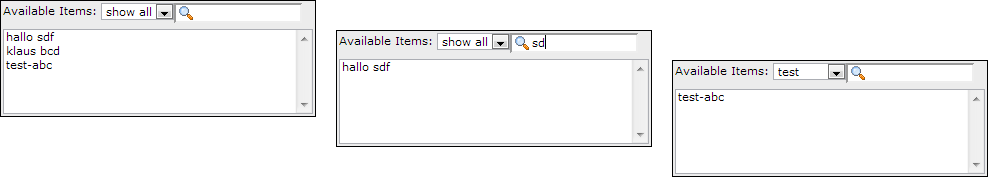
\includegraphics[width=1\linewidth]{Images/InDepthChanges/MultipleValueSelector.png}
	\end{figure}

\end{frame}

% ------------------------------------------------------------------------------
% Improved caching framework by introducing cache groups
% (slide added in March 2014)
% ------------------------------------------------------------------------------
% http://forge.typo3.org/issues/54991

\begin{frame}[fragile]
	\frametitle{Konceptualne izmene}
	\framesubtitle{Kes grupe (1)}

	\begin{itemize}
		\item TYPO3 core koristi dva tipa kesiranja:

			\begin{itemize}
				\item \textbf{system-related caches}:
				class loading cache, configuration cache, l10n\_cache, extbase\_object, extbase\_reflection etc.
				\item \textbf{frontend-related caches}:
				cHash cache, page cache, page section cache
			\end{itemize}

		\item U TYPO3 < 6.2, \textit{clear all caches} prazni \underline{sav} kes, sto nije idealno

		\item U TYPO3 >= 6.2, core koristi dve kes grupe:\newline
			"\textbf{pages}" sav kes koji se odnosi na kesiranje na strani i "\textbf{system}", kes koji se tice vremena za kompajliranje i konfigurisanje

	\end{itemize}

	\begin{figure}
		
\includegraphics[width=0.5\linewidth]{Images/InDepthChanges/CacheGroups.png}
	\end{figure}

\end{frame}

% ------------------------------------------------------------------------------
% Improved caching framework by introducing cache groups
% (slide added in March 2014)
% ------------------------------------------------------------------------------
% http://forge.typo3.org/issues/54991

\begin{frame}[fragile]
	\frametitle{Konceptualne izmene}
	\framesubtitle{Kes grupe (2)}

	\lstset{
		basicstyle=\tiny\ttfamily
	}

	\begin{itemize}

		\item Znacajna opcija za konfigurisanje:\newline
			\smaller(u fajlovima: \texttt{LocalConfiguration.php}/\texttt{DefaultConfiguration.php})\normalsize

			\begin{lstlisting}
			'cache_hash' => array(
			  'frontend' => 'TYPO3\CMS\Core\Cache\Frontend\VariableFrontend',
			  'backend' => 'TYPO3\CMS\Core\Cache\Backend\Typo3DatabaseBackend',
			  'options' => array(),
			  'groups' => array('pages', 'all')
			),
			\end{lstlisting}

		\item Komanda "\textit{Flush all caches}" vise ne brise system-related caches
			(samo "Clear Configuration Cache" ili Install Tool prazni ovakav tip kesa)
		\item Nova userTSconfig opcija omogucava da i neadministratori imaju mogucnost da ociste sistemski kes:\newline
			\smaller\texttt{options.clearCache.system = 1}\normalsize

		\breakingchange

	\end{itemize}

\end{frame}

% ------------------------------------------------------------------------------
% TCA: limit number of ticked checkboxes
% (slide added in March 2014)
% ------------------------------------------------------------------------------
% http://forge.typo3.org/issues/55187
% http://forge.typo3.org/issues/55188 (documentation: TCA reference)

\begin{frame}[fragile]
	\frametitle{Konceptualne izmene}
	\framesubtitle{TCA: Number of Ticked Checkboxes}

	\lstset{
		basicstyle=\tiny\ttfamily
	}

	\begin{itemize}
		\item TCA dozvoljava validaciju broja selektovanih cek boksova

			\begin{itemize}
				\item \texttt{maximumRecordsChecked}:\newline
					ogranicava broj zapisa system-wide
				\item \texttt{maximumRecordsCheckedInPid}:\newline
					ogranicava broj zapisa PID-wide (parent ID)
			\end{itemize}

		\item Ukoliko administrator prekoraci maksimalni broj, dodatno cekiranje se ponistava sve dok se neki drugi zapis ne odcekira

		\item Primer:

			\begin{lstlisting}
				$tcaConfiguration = array(
				  'type' => 'check',
				  'eval' => 'maximumRecordsChecked',
				  'validation' => array(
				    'maximumRecordsChecked' => 5
				  )
				);
			\end{lstlisting}

	\end{itemize}

\end{frame}

% ------------------------------------------------------------------------------
% TCA: Introduce MM_oppositeUsage property
% (slide added in March 2014)
% ------------------------------------------------------------------------------
% http://forge.typo3.org/issues/56061
% http://forge.typo3.org/issues/56123 (documentation: TCA reference)

\begin{frame}[fragile]
	\frametitle{Konceptualne izmene}
	\framesubtitle{TCA: \texttt{MM\_oppositeUsage} osobina}

	\lstset{
		basicstyle=\tiny\ttfamily
	}

	\begin{itemize}
		\item Prilikom kopiranja zapisa \texttt{sys\_category}, kreira se nova MM referenca, ali se tom prilikom ne postavlja "fieldname"
		\item Ova vrednost se u odnosu na suprotni entitet prosto definise sa \texttt{MM\_match\_fields}, ali joj se ne moze pristupiti
		\item Kako bi se razresio ovaj problem, uvodi se novi properti \texttt{MM\_oppositeUsage} za TCA:

			\begin{lstlisting}
				'config' => array(
				  'allowed' => '*',
				  'MM' => 'tx_myextension_first_second_mm',
				  'MM_oppositeUsage' => array(
				    'tt_content' => array('somefield'),
				    'tx_myextension_domain_model' => array('some_property'),
				  ),
				),
			\end{lstlisting}

	\end{itemize}

\end{frame}

% ------------------------------------------------------------------------------
% Miscellaneous
% ------------------------------------------------------------------------------
% http://forge.typo3.org/issues/49037 (Custom record list in element browser)
% http://forge.typo3.org/issues/36505 (Increase size of be_groups.subgroup field)
% http://forge.typo3.org/issues/49270 (Merge extensions TS/Template)

\begin{frame}[fragile]
	\frametitle{Konceptualne izmene}
	\framesubtitle{Razno}

	\begin{itemize}

		\item \textbf{Posebno prilagodjena lista rekorda:}\newline
			\small
				Posebno prilagodjena lista rekorda se moze koristiti u pretrazivacu elemenata i da pregazi pretpostavljenu listu
			\normalsize

		\item \textbf{Vise subgroups:}\newline
			\small
				Atribut \texttt{subgroup} u tabeli \texttt{be\_groups} promenjen je iz \texttt{varchar(250)} u \texttt{text}, sto omogucava vise podgrupa (administratori/administratorske grupe)
			\normalsize

		\item \textbf{Prosirenja TS/Template su integrisana:}\newline
			\small
				"WEB > Template" je bio podeljen u nekoliko prosirenja (tstemplate\_ceditor, tstemplate\_info, tstemplate\_objbrowser i tstemplate\_analyzer). Sada su ta prosirenja spojena u jedno pod nazivom "tstemplate"
			\normalsize

	\end{itemize}
	
\end{frame}

% ------------------------------------------------------------------------------
% Miscellaneous
% ------------------------------------------------------------------------------
% http://forge.typo3.org/issues/49721 (Add label_userFunc_options support to BackendUtility)
% http://forge.typo3.org/issues/50441 (Add a timestamp when downloading an extension)
% http://forge.typo3.org/issues/51352 (Force saltedpasswords for Backend)

\begin{frame}[fragile]
	\frametitle{Konceptualne izmene}
	\framesubtitle{Razno}

	\begin{itemize}

		\item \textbf{label\_userFunc\_options:}\newline
			\small
				Dodata podrska za \texttt{label\_userFunc\_options} u \texttt{BackendUtility}
			\normalsize

		\item \textbf{Naziv prosirenja:}\newline
			\small
				Kada se prosirenje preuzima iz Extension Manager-a, naziv prosirenja sadrzi timestamp (godina, mesec, dan i vreme):\newline
				\texttt{<extensionKey>\_<version>\_<timestamp>.zip}\newline
				\texttt{myextension\_1.0.0\_201312102359.zip}
			\normalsize

		\item \textbf{EXT:saltedpasswords:}\newline
			\small
				Prosirenje EXT:saltedpasswords je sada obavezno sistemsko prosirenje i odmah je aktivirano.
				Ovo forsira salted heširanje za autentifikaciju administratora. Install Tool proverava podesavanja i prilagodjava ih ukoliko je to neophodno.
			\normalsize

	\end{itemize}
	
\end{frame}

% ------------------------------------------------------------------------------
% Miscellaneous
% ------------------------------------------------------------------------------
% http://forge.typo3.org/issues/51138 (Allow SignalSlots to modify arguments)
% http://forge.typo3.org/issues/31996 (Transfer query parameters in preview)
% http://forge.typo3.org/issues/52630 (TCEforms PlaceHolder works recursively now)

\begin{frame}[fragile]
	\frametitle{Konceptualne izmene}
	\framesubtitle{Razno}

	\begin{itemize}

		\item \textbf{SignalSlots za modifikovanje argumenata:}\newline
			\small
				Argument prosledjen SignalSlots dispatcher-u može da se izmeni i sada dispatcher vraća (izmenjen) argument kao što ga je i primio da ne bi narušio uvezivanje.
			\normalsize

		\item \textbf{Workspace pregled:}\newline
			\small
				Parametri upita sada se prosledjuju workspace pregledu. Ovo je bio problem u TYPO3 < 6.2, gde su prosirenja prosledjivala posebno prilagodjene parametre koji nisu radili kako valja.
			\normalsize

		\item \textbf{TCEforms PlaceHolder funkcija:}\newline
			\small
				Uvedena u TYPO3 CMS 4.7, TCEforms funkcija, PlaceHolder, sada radi rekurzivno (npr. \texttt{\_\_row|uid\_foreign|field}).
			\normalsize

	\end{itemize}
	
\end{frame}

% ------------------------------------------------------------------------------
% Miscellaneous
% ------------------------------------------------------------------------------
% http://forge.typo3.org/issues/14730 (Support for proxy NTLM authentication)
% http://forge.typo3.org/issues/49667 (Enable double-resolution icons in SpriteGenerator)

\begin{frame}[fragile]
	\frametitle{Konceptualne izmene}
	\framesubtitle{Razno}

	\begin{itemize}

		\item \textbf{Ikonice u duploj rezoluciji:}\newline
			\small
				SpriteManager sada podrzava ikonice u visokoj rezoluciji: generise drugi sprite sa ikonicama u duploj velicini (drugi fajl sa sufiksom "@x2.png"). CSS3 se stara o tome da ikonice u visokoj rezoluciji budu prikazane na uredjajima koji ovo podrzavaju\newline
				(ne utice na performanse drugih uredjaja).
			\normalsize

		\item \textbf{Proxy NTLM autentifikacija:}\newline
			\small
				Dodata podrska za proxy NTLM autentifikaciju (\textbf{NT} \textbf{L}AN \textbf{M}anager: paket Microsoft sigurnosnih protokola) Ova mogucnost se moze aktivirati preko Install Tool-a:\newline
			\normalsize
			\smaller
				\texttt{\$GLOBALS['TYPO3\_CONF\_VARS']['SYS']['curlProxyNTLM']}\newline
				\emph{(mogucnost koja je zahtevana pre vise od 8 godina)}
			\normalsize

	\end{itemize}
	
\end{frame}

% ------------------------------------------------------------------------------
% Miscellaneous
% (slide added in March 2014)
% ------------------------------------------------------------------------------
% http://forge.typo3.org/issues/14730 (Support for proxy NTLM authentication)

\begin{frame}[fragile]
	\frametitle{Konceptualne izmene}
	\framesubtitle{Razno}

	\begin{itemize}

		\item \textbf{cookieHttpOnly kao osnovno podesavanje:}\newline
			\small
				Kako bi se session kolacicu moglo pristupiti samo kroz HTTP protokol, \texttt{cookieHttpOnly} je omoguceno kao osnovno podesavanje.\newline
				Ovo znaci da kolacicima, "fe\_typo\_user" i "be\_typo\_user" se vise nece moci pristupiti preko skript jezika (npr. JavaScript), sto pojacava zastitu protiv XSS napada (\textit{cross site scripting}). Neki stariji pretrazivaci ne podrzavaju ovu tehniku.
			\normalsize

		\item \textbf{Prociscene tabele u bazi podataka:}\newline
			\small
				Sledeci atributi su izbaceni iz tabela u bazi \texttt{tt\_content} (ne koristi se od TYPO3 4.0):
				\texttt{text\_align}, \texttt{text\_face}, \texttt{text\_size}, \texttt{text\_color}, \texttt{text\_properties}.
			\normalsize

	\end{itemize}
	
\end{frame}

% ------------------------------------------------------------------------------
% Miscellaneous
% (slide added in March 2014)
% ------------------------------------------------------------------------------
% https://forge.typo3.org/issues/55190 (Move Tidy functionality to a TER extension)

\begin{frame}[fragile]
	\frametitle{Konceptualne izmene}
	\framesubtitle{Razno}

	\begin{itemize}

		\item \textbf{HTML Tidy uklonjeno:}\newline
			\small
				Funkcionalnost \textit{HTML Tidy} je uklonjena iz TYPO3 core. Moze se lako ponovo pokrenuti instalacijom EXT:tidy iz TER.
			\normalsize

		\item \textbf{dontSetCookie uklonjeno:}\newline
			\small
				Zbog cinjenice da se kolacic "fe\_typo\_user" podesava samo ako je potreban (ne uvek), the Install Tool opcija \texttt{dontSetCookie} je postala suvisna i samim tim je uklonjena.
			\normalsize

		\item \textbf{"Wizard" scripts uklonjeno:}\newline
			\small
				Sledeci "wizard" scripts su uklonjeni:
				\texttt{typo3/wizard\_add.php}, \texttt{typo3/wizard\_colorpicker.php}, \texttt{typo3/wizard\_edit.php}, \texttt{typo3/wizard\_forms.php}, \texttt{typo3/wizard\_list.php}, \texttt{typo3/wizard\_rte.php}, \texttt{typo3/wizard\_table.php}
			\normalsize

	\end{itemize}
	
\end{frame}

% ------------------------------------------------------------------------------

